\chapter[Opis projektu]{Opis projektu}

\section[Treść zadania]{Treść zadania}

\par{Zaprojektować i zaimplementować usługę udostępniania danych statystycznych na temat studentów uczelni wyższej, przy założeniu bezpiecznej i niezawodnej dystrybucji danych wrażliwych - poufnych informacji o studentach.}

\par{Usługa powinna:}
\begin{itemize}


\item mieć dokładnie jeden ten sam tekstowy plik konfiguracyjny dla części 
serwerowej i klientów usługi,
\item składać się po stronie serwerowej z dwóch warstw: (1)  wewnętrznej
  wytwarzającej, przechowującej i przesyłającej przetworzoną wrażliwą
informację, (2) warstwy zewnętrznej do udostępniania przetworzonej informacji
oprogramowaniu klienckiemu usługi,
\item oprogramowanie realizujące część serwerową powinno być współbieżne,
\item składać się po stronie klienckiej z prostych narzędzi opatulających
  zaproponowane API protokołu komunikacyjnego,
\item zapewniać odporność na uszkodzenia węzła, stąd każda z warstw powinna być
  uruchomiona na co najmniej dwóch węzłach,
\item zapewniać realizację usługi w trakcie awarii w czasie obsługi,
\item obsługiwać scenariusz próby ponownego wpięcia się przez węzeł dowolnej z
  warstw, z którym wcześniej utracono łączność, a zarazem być odporną na próbę
zastąpienia nieosiągalnego sieciowo węzła (np. w wyniku ataku DoS, odmowa
usługi) węzłem wrogim do tego nieuprawnionym,
\item na bieżąco i transparentnie dla oprogramowania klienckiego zarządzać
  dostępnymi zasobami lokalizacyjnymi,
\item zapewniać zadany (większy niż 1 ale dopuszczalny konfiguracją mniejszy niż
  liczba serwerów danych) poziom redundancji - z obsługą uzupełniania kopii na
innych serwerach w przypadku awarii włącznie,
\item cała część sewerowa usługi powinna być uruchamiana i zamykana jednokrotnym
  wywołaniem skryptu na jednym węźle serwera z jednym argumentem
<start|stop|status> (wykorzystanie nieinteraktywnych metod automatycznego
uwierzytelniania węzłów w SSH).

\end{itemize}

\section[Ogólny opis rozwiązania]{Ogólny opis rozwiązania}

\par{Nasze rozwiązanie to rozproszony system do rejestracji na przedmioty studentów uczelni wyższej. Warstwą wewnętrzną przechowujące dane wrażliwe, w tym przypadku będą węzły rejestrujące studentów, ideowo umieszczone w dziekanatach instytutów i obsługiwane przez osoby tam pracujące. Warstwa pośrednia przechowuje informacje o studentach, jednak bez informacji wrażliwej. Posiada jedynie dane o istnieniu studenta zapisanego na przedmioty, bez imienia, nazwiska i daty urodzenia. Owe informacje są przetwarzane na żądanie aplikacji klienckiej, dostępnej dla studentów, którzy chcą dowiedzieć się, ile osób zapisanych jest na dany przedmiot.}

\subsection[Dane wrażliwe a kwestie prawne]{Dane wrażliwe a kwestie prawne}

\par{W związku z ochroną danych wrażliwych zapoznaliśmy się z Ustawą o ochronie danych osobowych z dnia 29 sierpnia 1997 r. Pomimo, że generowane przez nas w ramach projektu losowe dane, nie zawierają faktycznych wrażliwych informacji, przystosowaliśmy nasz system do obowiązującego w Polsce prawa, pod uwagę biorąc przede wszystkim poniższe kwestie prawne z Ustawy o ochronie danych osobowych:}
\begin{itemize}
\item Art. 2 \textit{,,Ustawę stosuje się do przetwarzania danych osobowych (...) w systemach informatycznych, także w przypadku przetwarzania danych poza zbiorem danych.''}s
\item Art. 6 \textit{,,W rozumieniu ustawy za dane osobowe uważa się wszelkie informacje dotyczące zidentyfikowanej lub możliwej do zidentyfikowania osoby fizycznej.''}
\item Art. 6 \textit{,,Informacji nie uważa się za umożliwiającą określenie tożsamości osoby, jeżeli wymagałoby to nadmiernych kosztów, czasu lub działań.''}
\item Informacje o Generalnym Inspektorze w Art. 14 i Art. 16.
\item Informacje na temat ochrony danych w Art. 26 oraz Art. 26a.
\item Informacje o uprawnieniach administratora w Art. 31.
\item Informacje o zabezpieczeniu danych osobowych z rozdziału 5.
\end{itemize}

\section[Projekt architektury]{Projekt architektury}

\par{Wewnętrzna warstwa serwera wytwarza i przechowuje informacje na temat studentów uczelni wyższej - stworzone na podstawie danych wprowadzonych przez pracowników dziekanatu. Następnie owa warstwa przesyła informacje do warstwy zewnętrznej serwera (warstwy przetwarzającej) świadczącej usługi udostępniania informacji przetworzonej rozwiązaniom klienckim. Każda z warstw komunikować się będzie z użyciem protokołu TCP/IP przesyłając wiadomości zserializowane za pomocą Google Protocols Buffer.}

\begin{figure}[h!tb]
\begin{center}
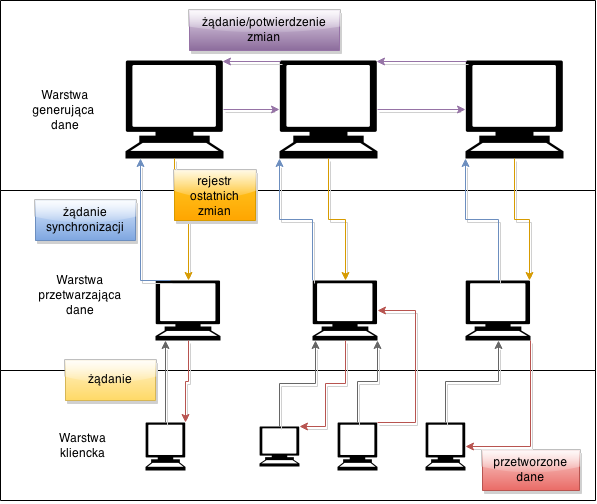
\includegraphics[width=0.9\linewidth]{img/dane_net.png} 
\caption{Diagram ilustrujący komunikację pomiędzy poszczególnymi warstwami}
\label{img:dane_net}
\end{center}
\end{figure}

\subsection[Warstwa wewnętrzna serwera][Warstwa wewnętrzna serwera]{Warstwa wewnętrzna serwera}

\par{Warstwa stworzona w technologii token ring. Węzły połączone są w pierścień i przesyłają sobie kolejno token zawierający informacje o potencjalnych zmianach. Tylko węzeł posiadający token może wykonywać operację aktualizacji danych. Każda zmiana musi być zatwierdzona przez pozostałe węzły. Zapewnia to synchronizację danych oraz bieżące sprawdzenie działania pozostałych węzłów.}

\par{Dane wrażliwe przechowywane są w postaci rekordów zawierających:}

\begin{itemize}
\item ID studenta
\item imię studenta
\item nazwisko studenta
\item datę urodzenia
\item listę przedmiotów na jakie jest zapisany
\end{itemize}

\subsubsection*[Opis szczegółowy]{Opis szczegółowy}


\par{W momencie podłączania węzeł wewnętrzny wysyła wiadomość z chęcią zalogowania się do sieci do jednego z innych węzłów z listy znajdującej się w pliku konfiguracyjnym. Robi tak aż do skutku, tzn. dopóki nie dostanie wiadomości od któregokolwiek innych węzłów z informacją o włączeniu się do sieci. Jeśli jednak mimo wszystkich prób nie dostanie wiadomości - uznaje, że jest pierwszym węzłem w sieci. Jest to rozwiązanie czasochłonne, niemniej będzie ono miało miejsce bardzo rzadko, ze względu na ogólnie przyjętą zasadę, że warstwa wewnętrzna działa nieprzerwanie i wymaga przynajmniej 3 aktywnych węzłów do poprawnego działania.}

\par{Węzły w tej warstwie wysyłają sobie kolejno token po okręgu, tzn. kiedy węzeł dostaje token wprowadza odpowiednią aktualizację (nie zawsze!) oraz przesyła go dalej). Token zawiera w sobie informację o stanie, w którym znajduje się sieć, a także obraz jej topologii (następujące po sobie węzły). Dzięki temu można zapewnić stały stan sieci dla wszystkich węzłów. Z każdą kolejną operacją (zatwierdzoną przez wszystkie węzły) stan sieci zwiększa się o jeden. Zasady są następujące:
\begin{itemize}
\item Jeśli stan jest większy od posiadanego przez węzeł, następuje zapis nowego stan i przesłanie do następnego węzła.
\item Jeśli stan jest równy posiadanemu i nie jest on ustawiony przez ten węzeł, to może on wykonać swoją operację (zwiększając stan o 1).
\item Jeśli stan jest równy posiadanemu i jest on ustawiony przez ten węzeł, oznacza to, że ostatnia operacja wygenerowana przez ten węzeł została zaakceptowana przez sieć.
\item Jeśli stan jest mniejszy od posiadanego, token jest ignorowany.
\end{itemize}

\par{Jeśli token jest oznaczony jako ,,wolny'' (przypadek 2 z powyższej listy) dany węzeł może użyć go do wprowadzenia nowych danych, nowego węzła do sieci bądź odpytania o aktualność danych. Następnie węzeł czeka na powrót tokena z odpowiedzią i po jej uzyskaniu podaje go dalej. Dzięki temu, że węzeł nie może użyć tokena od razu po poprzednim zadaniu, które wygenerował, eliminujemy problem zagłodzenia innych węzłów. Ponadto poprzez ruch tokena po pierścieniu możemy w łatwy sposób ,,ustalać'' dane decyzje z innymi węzłami oraz sprawdzać ich aktywność.}

\par{W przypadku zerwania połączenia z następnikiem wykonywane są kolejne operacje:}
\begin{itemize}
\item Usuwanie następnika z topologii sieci w stanie, który aktualnie węzeł posiada.
\item Zwiększenie stanu o 2.
\item Połączenie się ze swoim nowym następnikiem.
\item Przesłanie stanu do następnika (generacja tokena).
\end{itemize}

\par{W sytuacji awarii węzeł automatycznie generuje token, a poprzedni staje się nieaktualny i wkrótce zostanie usunięty z sieci. Cecha generowania tokena powoduje, że zostanie on zawsze odtworzony w sieci niezależnie od tego czy awarii ulegnie węzeł, który go posiadał czy dowolny inny.}

\par{Należy pamiętać, że w trakcie zapisywania stanu trzeba sprawdzić, czy nie zmienił się nasz następnik w topologii sieci. Jest to szczególnie istotne w przypadku jednoczesnej awarii wielu węzłów, gdy wiele węzłów wygeneruje nowe tokeny. Jeden z nich zdominuje sieć, a drugi będzie zmuszony do ponownego sprawdzenia braku połączenia ze swoim dawnym następnikiem i ponownego wymuszenia zmiany topologii sieci. Takie rozwiązania zwiększa czas przywracania sieci do działania przy awarii wielu węzłów jednocześnie, niemniej zapewnia spójność jej stanu i istnienie w stanie ustalonym tylko jednego ważnego tokena.}


\subsection[Warstwa zewnętrzna serwera]{Warstwa zewnętrzna serwera (warstwa przetwarzająca)}

\par{Warstwa przeznaczona do komunikacji z aplikacją kliencką. Na żądanie klienta przetwarza wcześniej otrzymane od warstwy wewnętrznej dane i wynik przetwarzania zwraca klientowi. Moduł ten synchronizuje dane okresowo (częstość jest ustalana w pliku konfiguracyjnym), tak aby administrator sam był wstanie dostosować interwał do aktualnych potrzeb).}

\par{Dane o studentach przechowywane są w poniższej postaci:}

\begin{itemize}
\item ID studenta
\item listę przedmiotów na jakie jest zapisany
\end{itemize}

\subsubsection*[Opis szczegółowy]{Opis szczegółowy}
\par{Serwer zewnętrzny w momencie logowania wysyła Heartbeata do wszystkich serwerów z listy ustalonej w pliku konfiguracyjnym. Węzły, które mu odpowiedzą serwer uznaje za aktywne w danej chwili. Dzięki temu zyskuje obraz aktywnych węzłów w warstwie. Od tej pory co ustalony interwał wysyła wiadomość do każdego z tych serwerów. Jeśli otrzyma TestRequesta od węzła uznawanego do tej pory za nieaktywny, dodaje go do listy aktywnych oraz zaczyna wysyłać mu Heartbeaty. W momencie, gdy czas oczekiwania na Heartbeat przekracza ustalony interwał wysyłany jest TestRequest wymuszający odpowiedź Heartbeatem. Gdy i to zawiedzie węzeł uznany jest za nieaktywny.}

\par{W określonych w pliku konfiguracyjnym interwałach czasu serwer zewnętrzny pobiera dane od serwera wewnętrznego, zapisując je w swojej bazie w bezpiecznej formie (bez danych wrażliwych). Jeśli dany węzeł wewnętrzny nie odpowie - próbuje z kolejnym, itd.}

\par{W Heartbeatach przesyłana jest informacja o ilości podłączonych w danej chwili klientów.}

\par{Każdy węzeł utrzymuje dane na temat podłączonych do niego klientów oraz klientów podłączonych do pozostałych aktywnych węzłów. Dzięki temu można zapewnić równomierne obciążenie między węzłami serwera. Jeśli dany serwer dostanie wiadomość o chęci zalogowania się nowego klienta sprawdza czy inny serwer nie ma mniej klientów od niego (o więcej niż 2). Jeśli tak - przełącza klienta na inny serwer. Algorytm ten został szerzej opisany w opisie szczegółowym aplikacji klienckiej.}

\par{Nie jest potrzebne stałe sprawdzanie aktywności serwerów z warstwy wewnętrznej, ze względu na możliwe długie interwały czasowe między synchronizacją (np. jeden dzień). W przypadku częstszych synchronizacji (np. co minutę) sprawdzanie aktywności wewnętrznego węzła będzie i tak sprawdzane na bieżąco. W trakcie synchronizacji nie jest pobierana cała baza, a jedynie zmiany od ostatniej zgodności. Dokładnie cały algorytm został opisany w rozdziale ,,Sposób synchronizacji danych między warstwą zewnętrzną a wewnętrzną''.}

\par{W momencie otrzymania wiadomości od klienta z danym żądaniem wykonywane są wymagane obliczenia i wysyłana odpowiedź.}


\subsection[Aplikacja kliencka]{Aplikacja kliencka}

\par{Warstwa przeznaczona dla klienta to z założenia lekka i intuicyjna aplikacja konsolowa. Moduł ten bezpośrednio łączyć będzie się tylko z modułem zewnętrznym serwera. Użytkownik, za pomocą tej aplikacji będzie mógł dowiedzieć się ile osób w danym momencie jest zapisany na wybranie przez niego przedmiot. Aplikacja będzie działała synchronicznie, tzn. po wysłaniu żądania będzie się zawieszała w oczekiwaniu na odpowiedź.}

\subsubsection*[Opis szczegółowy]{Opis szczegółowy}
\par{Każda aplikacja kliencka w momencie uruchomienia stara się połączyć do jednego z serwerów zewnętrznych. Lista serwerów jest z góry ustalona i znajduje się pliku konfiguracyjnym. Klient próbuje zestawić połączenie najpierw z pierwszym serwerem z listy, czekając 10 sekund na odpowiedź. W razie jej braku próbuje tego z kolejnym serwerem, itd. Jeśli klientowi uda się połączyć serwerem, jednak ten ,,stwierdzi'', że obsługuje zbyt dużą ilość klientów w stosunku do pozostałych węzłów, wtedy wysyła on wiadomość zwrotną z informacją, do którego serwera klient ma się podłączyć. Następuje, więc ponowna próba połączenia, tym razem z polecanym węzłem. Cała operacja jest ,,ukryta'' przed użytkownikiem aplikacji klienckiej, tzn. nie wie on, do którego serwera się podłącza.}

\par{Od momentu zestawienia połączenia klient może wysyłać żądania do serwera. Po wysłaniu żądania czeka na odpowiedź. Po jej otrzymaniu może wysłać kolejne żądanie. Ponadto co ustalony interwał klient wysyła Hearbeat do serwera dając znać, że ciągle jest podłączony. Analogicznie serwer informuje klienta, że działa poprawnie.}

\par{W razie awarii bądź braku odpowiedzi od serwera wysyłany jest TestRequest wymuszający wysłanie Heartbeata. Jeśli mimo to serwer nie odpowiada następuje próba zestawienia połączenia z kolejnym serwerem z listy.}


\subsection[Sposób synchronizacji danych między warstwami]{Sposób synchronizacji danych między warstwami}

\textit{\textbf{TODO}}

\section[Wymagania i założenia]{Wymagania i założenia}

\subsection[Wymagania funkcjonalne]{Wymagania funkcjonalne}

\begin{tabularx}{\textwidth}{|c|X|X|}
\hline
\textbf{ID} & \textbf{Wymagania}  & \textbf{Powody decyzji} \\
\hline

\label{z:WF1} WF1 & \textbf{Plik konfiguracyjny}


Każdy z węzłów danej warstwy będzie posiadała plik konfiguracyjny o tej samej strukturze. W zależności od typu dane z pliku zostaną odpowiednio skonfigurowane. Plik będzie zawierał: ID węzła, listę serwerów (zależnie od typu - zewnętrznych lub wewnętrznych), dodatkowe dane konfiguracyjne (np. odpowiadających za redundancję danych, okresową synchronizację, itd.) &
Takie rozwiązanie jest wymagane w treści zadania. Ponadto ujednolica i ułatwia konfigurację projektu bez potrzeby ponownej kompilacji.\\
\hline

\label{z:WF2} WF2 &  \textbf{Zmiana jednego rekordu na raz }

Jeśli dany węzeł chce dodać/usunąć/zmodyfikować dane o studencie musi posiadać token, który przesyła do kolejnych serwerów na końcu otrzymując potwierdzenie, że każdy z węzłów wprowadził żądaną zmianę. & 
Ze względu na to, że w sieci warstwy wewnętrznej serwera istnieje jeden token jest sensowne przyjąć założenie, że na raz można wprowadzić jedną modyfikację w bazie. Ponadto pozwala to utrzymać nieduży rozmiar tokena, co sprzyja jego szybszemu przesyłaniu między węzłami. Nawet w przypadku wielu żądań (od każdego węzła jedno) powinno to działać na tyle szybko, że osoby wprowadzające dane nie odczują opóźnienia. Dodatkowo wprowadzanie pojedynczych informacji pozwala na szybsze wykrycie awarii węzła serwera oraz zaoszczędza więcej czasu, niż w przypadku wpisywania dużej ilości danych na raz, a dopiero potem sprawdzania czy węzeł działa poprawnie. \\
\hline

\end{tabularx}
\newpage
\begin{tabularx}{\textwidth}{|c|X|X|}
\hline
\textbf{ID} & \textbf{Wymagania}  & \textbf{Powody decyzji} \\
\hline

\label{z:WF3} WF3 & \textbf{Okresowa synchronizacja}

 Synchronizacja z warstwą wewnętrzną następuje okresowo, w danych odstępach czasu, sterowanych za pomocą pliku konfiguracyjnego. Jest ona wykonywana na rządanie węzłów warstwy zewnętrznej. Synchronizacja polega na pobraniu jedynie zmienionych rekordów bazy, a nie wszystkich. Ostatnia funkcjonalność zostanie rozwiązana za pomocą, tzw. ,,znaczników czasu'' \textit{(ang. timestamp)}. & Synchronizacja o konkretnych porach pozwala na odpowiednie rozporządzanie pracą systemu. W przypadku rzadkiej modyfikacji danych przez warstwę wewnętrzną serwera synchronizacja może być wykonywana, np. raz na dzień. Z drugiej strony można ustawić synchronizację co 1 sekundę, co spowoduje wrażenie ciągłej synchronizacji (oczywiście nie biorąc pod uwagę potencjalnych opóźnień). Takie rozwiązanie pozwala administratorowi na odpowiednią optymalizację działania systemu. Dzięki aktualizacji jedynie konkretnych danych, a nie bazy w całości jest to stosunkowo szybkie. \\
\hline

\label{z:WF4} WF4 & \textbf{Redundancja danych (warstwa wewnętrzna serwera)}

W zależności od zmiennej ustawionej w pliku konfiguracyjnym warstwa wewnętrzna może posiadać pełną redundancję bądź nie. Przyjmuje się, że minimalna liczba serwerów posiadających w pełni aktualne dane to 3. & To założenie służy spełnieniu warunków zadania. Możliwość modyfikacji poziomu redundancji pozwala dopasować system do ilości węzłów w warstwie wewnętrznej serwera i do danego zapotrzebowania.\\
\hline

\label{z:WF5} WF5 & \textbf{Udostępnianie usług }

 Warstwa zewnętrzna obsługuje żądania klientów realizując usługę zwracania ilości studentów zapisanych na dany przedmiot. Serwer nasłuchuje czekając na żądania, a następnie (w ramach możliwości) je spełnia. & To założenie służy spełnieniu warunków zadania. \\
\hline



\label{z:WF6} WF6 & \textbf{Obliczanie danych statystycznych }

  Serwery zewnętrzne, zwane też przetwarzającymi, otrzymują dane od warstwy wewnętrznej, jednak zapisują z nich jedynie dane niewrażliwe używając ich do wyliczania ilości studentów zapisanych na dany przedmiot. Do tej operacji pełne informacje o studentach nie są potrzebne. & 
To założenie służy spełnieniu warunków zadania. \\
\hline

\end{tabularx}
\newpage
\begin{tabularx}{\textwidth}{|c|X|X|}
\hline
\textbf{ID} & \textbf{Wymagania}  & \textbf{Powody decyzji} \\
\hline

\label{z:WF7} WF7 & \textbf{Dostęp do usługi pobrania danych statystycznych} 
 
Aplikacja kliencka po połączeniu z serwerem zewnętrznym może pobrać informacje na temat ilości studentów zapisanych na dany przedmiot. Użytkownik otrzymuje jedynie nazwę przedmiotu i liczbę zapisanych studentów, bez dostępu do danych wrażliwych. Może być wysyłane jedno żądanie na raz od danego użytkownika. Nie ma funkcji agregacji wiele żądań w jedno. & 
Jest to dobry przykład funkcjonalności, która zabezpiecza nam dane wrażliwe przed zwyczajnym użytkownikiem, udostępniając jedynie informacje, które mogą być publiczne. Agregacja bądź wysyłanie wielu żądań na raz nie jest konieczne do sprawdzenia poprawnego działania systemu i nie zmienia w żaden sposób wizji jego funkcjonowania.\\
\hline



\end{tabularx}

\subsection[Wymagania niefunkcjonalne]{Wymagania niefunkcjonalne}


\begin{tabularx}{\textwidth}{|c|X|c|}
\hline
\textbf{ID} & \textbf{Wymaganie}  & \textbf{Priorytet} \\
\hline

\label{z:WNF1} WNF1 & \textbf{Czas między awariami} 
 
Średni czas między awariami systemu powinien wynosić przynajmniej trzy miesiące, przy czym awarię definiujemy jako ciągłą niedostępność usługi przez co najmniej 10 minut bądź konieczność wykorzystania kopii zapasowej
 & bardzo wysoki\\
\hline

\label{z:WNF2} WNF2 & \textbf{Spójność danych po awarii} 
 
Odzyskane dane nie mogą być starsze niż 6 godzin przed awarią.
 & bardzo wysoki\\
\hline

\label{z:WNF4} WNF4 & \textbf{Ochrona danych} 
 
System powinien gwarantować ochronę danych osobowych studentów.
 & bardzo wysoki\\
\hline

\label{z:WNF5} WNF5 & \textbf{Czas naprawy} 
 
Maksymalny czas niesprawności systemu po awarii nie może przekraczać 2 godzin.
 & bardzo wysoki\\
\hline

\label{z:WNF6} WNF6 & \textbf{Czas odpowiedzi klientowi} 
 
Średni czas odpowiedzi klientowi na zapytanie, nie powinien trwać więcej niż  2 sekundy.
 & średni\\
\hline

\label{z:WNF7} WNF7 & \textbf{Maksymalny napływ studentów} 
 
Maksymalny przypływ nowych studentów do rejestracji nie powinien być większy niż 10 na sekundę.
 & średni\\
\hline

\label{z:WNF8} WNF8 & \textbf{Średni napływ studentów} 
 
Średni przypływ nowych studentów do rejestracji nie powinien być większy niż 5 na sekundę.
 & średni\\
\hline

\label{z:WNF9} WNF9 & \textbf{Dostępność} 
 
Średni czas wyłączenia systemu w roku nie powinien przekraczać dwóch dni roboczych.
 & wysoki\\
\hline

\label{z:WNF10} WNF10 & \textbf{Ergonomia} 
 
Użytkowanie systemu powinno być intuicyjne i przejrzyste dla użytkownika.
 & wysoki\\
\hline

\label{z:WNF11} WNF11 & \textbf{Praca po awarii węzła} 
 
Awaria pojedyńczego węzła nie powinna powodować awarii całej sieci (przy założeniu, że zachowana zostaje minimalna ilość węzłów).
 & bardzo wysoki\\
\hline

\label{z:WNF12} WNF12 & \textbf{Minimalna ilość węzłów do pracy warstwy wewnętrznej} 
 
Warstwa wewnętrzna serwera przechowująca dane powinna poprawnie działać przy minimalnej liczbie węzłów trzy. Jeśli liczba węzłów po awarii spadnie poniżej tej liczby, poprawne działanie nie jest gwarantowane.
 & bardzo wysoki\\
\hline

\label{z:WNF13} WNF13 & \textbf{Minimalna ilość węzłów do pracy warstwy zewnętrznej} 
 
Warstwa zewnętrzna serwera przetwarzające dane powinna poprawnie działać jeśli działa przynajmniej jeden węzeł tej warstwy.
 & bardzo wysoki\\
\hline

\label{z:WNF14} WNF14 & \textbf{Pomoc} 
 
System powinien posiadać dobrze przygotowaną pomoc dla użytkownika.
 & niski \\
\hline

\end{tabularx}


\subsection[Dodatkowe założenia]{Dodatkowe założenia}

\begin{tabularx}{\textwidth}{|c|X|X|}
\hline
\textbf{ID} & \textbf{Wymagania}  & \textbf{Powody decyzji} \\
\hline

\label{z:ZO1} ZO1 &  \textbf{Protokół TCP/IP }

Komunikacja między warstwami (wewnętrzna serwera - zewnętrzna serwera jak i zewnętrzna serwera - klienci) odbywa się za pomocą protokołów TCP/IP, wykorzystując Google Protocol Buffer (więcej w podrozdziale \ref{protobuf}). & 
Protokół został przez nas wybrany ze względu na elastyczność dla różnych konfiguracji serwerów, tzn. bez względu na to czy warstwy serwera będą działały w obrębie jednego węzła czy nie protokół pozwoli na poprawną komunikację. W przypadku działania obu warstw serwera na jednym komputerze czy nawet w jednym procesie wydajność będzie mniejsza (w porównaniu np. do pamięci współdzielonej), jednak ze względu na ograniczony czas projektu i mniejsze skomplikowanie zostało wybrane to rozwiązanie. \\
\hline

\label{z:ZO2} ZO2 &  \textbf{Proste komendy serwera}

Warstwy serwera będą uruchamiane i zamykane jednokrotnym wywołaniem skryptu na danym węźle serwera z jednym argumentem: start, stop oraz status, które będą kolejno: uruchamiać usługi serwera, wyłączać usługi serwera oraz wyświetlać status serwera. & 
Takie rozwiązanie jest wymagane w treści zadania. Ponadto pozwoli na łatwą obsługę i testowanie części serwerowej systemu. \\
\hline

\label{z:ZO3} ZO3 &  \textbf{Technologia token ring (warstwa wewnętrzna serwera)}

Serwery warstwy wewnętrznej połączone są ze sobą w pierścień (każdy ma z góry ustalonego poprzednika i następnika w pliku konfiguracyjnym). Jeśli dany następnik nie odpowiada - brany jest następny adres węzła z listy. W ten sposób bez względu na ilość węzłów mamy zawsze do czynienia z taką samą strukturą (w szczególności - mamy tylko jeden węzeł). Każdy z węzłów wysyła swojemu następnikowi token zawierający informacje odnośnie potencjalnych zmian. & 
Taka architektura warstwy wewnętrznej pozwala na bieżące sprawdzanie stanu kolejnych węzłów. Jeśli token gdzieś się ,,zagubi'' oznacza to, że dany węzeł uległ awarii. Ponadto taka architektura pozwala na szybką i łatwą synchronizację danych. \\
\hline

\end{tabularx}

\pagebreak

\begin{tabularx}{\textwidth}{|c|X|X|}
\hline
\textbf{ID} & \textbf{Wymagania}  & \textbf{Powody decyzji} \\
\hline
\label{z:ZO4} ZO4 &  \textbf{Pełna redundacja danych (warstwa zewnętrzna serwera)}

Każdy z węzłów zewnętrznych ma pełne i aktualne dane. Są one synchronizowane na bieżąco. & 
Natychmiastowa synchronizacja danych i pełna redundancja pozwala uniknąć wielu problemów w trakcie działania serwera, między innymi: dodatkowej synchronizacji po awarii jednego z węzłów, która jest dość problematyczna i skomplikowana. Rozwiązanie to zostało zatwierdzone przez Prowadzącego.\\
\hline

\label{z:ZO5} ZO5 &  \textbf{Wysyłanie ,,heartbeatów'' (warstwa zewnętrzna serwera/aplikacja kliencka)}

Węzły zewnętrznej warstwy będą sprawdzały swoją dostępność za pomocą tzw. ,,uderzeń serca'' \textit{(ang. heartbeat)} wysyłanych w danych odstępach czasu (każdy z serwerów musi mieć ustalony ten sam interwał). Dzięki temu będą miały wiedzę na temat aktywności pozostałych serwerów. Brak ,,heartbeata'' od danego serwera po upływie zadanego czasu będzie równoważny z jego brakiem dostępności. To samo tyczy się połączenia klient - serwer zewnętrzny. & 
Takie rozwiązanie pozwala na bieżąco monitorować stan poszczególnych węzłów warstwy zewnętrznej oraz ilość podłączonych klientów. \\
\hline

\label{z:ZO6} ZO6 &  \textbf{Brak funkcji logowania użytkownika}

Klient łączy się z systemem identyfikując się jedynie swoim unikatowym ID, które wpisane jest pliku konfiguracyjnym. & 
Decyzja została zatwierdzona przez Prowadzącego. Wynika ona z braku konieczności stworzenia tej funkcjonalności (w związku z minimalnym wpływem na główny cel projektu) oraz na ograniczony czas i mniejszą ilość osób w grupie projektowej niż przewidywana.  \\
\hline

\label{z:ZO7} ZO7 &  \textbf{Brak interfejsu graficznego (aplikacja kliencka)}

- & 
Decyzja została zatwierdzona przez Prowadzącego. Wynika ona z braku konieczności stworzenia tej funkcjonalności (w związku z minimalnym wpływem na główny cel projektu) oraz na ograniczony czas i mniejszą ilość osób w grupie projektowej niż przewidywana.
\\
\hline
\label{z:ZO8} ZO8 &  \textbf{Komunikacja synchroniczna (aplikacja kliencka)}

Aplikacja kliencka będzie się komunikowała z serwerem w sposób asynchroniczny. & 
Ze względu na ograniczoną funkcjonalność aplikacji klienckiej, sprowadzoną jedynie do wysyłania żądań i uzyskiwania odpowiedzi, ten sposób komunikacji wydaje się najbardziej trafny. Jedyna dodatkowa funkcjonalność klienta to wysyłanie co określony interwał czasu Heartbeatów dających znać, że klient jest ciągle podłączony.\\
\hline

\end{tabularx}

\pagebreak

\begin{tabularx}{\textwidth}{|c|X|X|}
\hline
\textbf{ID} & \textbf{Wymagania}  & \textbf{Powody decyzji} \\
\hline
\label{z:ZO9} ZO9 &  \textbf{Brak funkcji ,,heartbeatu'' (aplikacja kliencka)}

Aplikacja kliencka nie będzie na bieżąco sprawdzała stanu węzła do którego jest podłączona. Status serwera będzie przez nią sprawdzany jedynie przy logowaniu i wysyłaniu żądania. W przypadku awarii węzła aplikacja będzie przełączała się na kolejny węzeł z listy, aż do skutku. & 
Ze względu na naszą koncepcję aplikacji klienckiej ta funkcjonalność nie jest potrzebna. Z punktu widzenia użytkownika stan serwera interesuje go tylko przy wysyłaniu żądania. System heartbeatów dodaje duży narzut i komplikuje samego klienta nie dając w zamian znacznego wzrostu szybkości działania. W sytuacji awarii i tak musi nastąpić przełączenie na inny węzeł. Różnica polega jedynie na tym, że w przypadku systemu hearbeatów następuje to w momencie upływu określonego czasu bez odpowiedzi serwera, a w przeciwnym - jedynie wtedy kiedy serwer jest potrzebny, tzn. przy logowaniu bądź wysłaniu żądania.\\
\hline

\label{z:ZO10} ZO10 &  \textbf{Brak interaktywności (aplikacja kliencka)}

Aplikacja kliencka będzie ograniczona jedynie do wywoływania określonych funkcji, według określonego z góry scenariusza. & 
W związku z ograniczonym czasem i głównym celem projektu interaktywna aplikacja kliencka nie jest koniecznością. Funkcjonalność systemu można poprawnie przetestować inicjując konkretne scenariusze (między innymi symulacje awarii czy błędów systemu). Decyzja ta została zatwierdzona przez Prowadzącego.\\
\hline

\end{tabularx}

\section[Struktura systemu]{Struktura systemu}

\subsection{Struktura tokena}
\begin{lstlisting}
enum TokenType {
    NONE = 0;
    UPDATE = 1;
    CHECK = 2;
    ENTRY = 3;
}

message Person {
    required string uuid = 1;
    optional string name = 2;
    optional string surname = 3;
    optional int32 birthDate = 4;
    required int64 timestamp = 5;
}

message PersonSubject{
    required string uuid = 1;
    required string UUIDPerson = 2;
    required string UUIDSubject = 3;
    required int64 timestamp = 4;
}

message Subject{
    required string uuid = 1;
	required string name = 2;
	required int64 timestamp = 3;
}

message Token{
    required TokenType tokenType = 1;
    optional int32 serverId = 2;
    repeated int32 nodeIds = 3;
    optional int64 timespamp = 4;
}
\end{lstlisting}

\subsection[Struktura wiadomości]{Struktura wiadomości}
\begin{lstlisting}
message EntityState{
    repeated Person students = 1;
    repeated PersonSubject personSubjects = 2;
    repeated Subject subjects = 3;
}

message MiddlewareRequest{
	required int32 nodeId= 4;
    required int64 timestamp = 1;
}

message MiddlewareResponse{
    required EntityState changes = 1;
}

enum MiddlewareMessageType{
    Request = 0;
    Response = 1;
    Redirect = 2;
    Heartbeat = 3;
}

message MiddlewareMessage{
	required int32 nodeId= 2;
    optional string subjectName = 3;
    optional int32 registeredStudents = 4;    
}

message MiddlewareHeartbeat{
    required int32 serverId = 1;
    optional int32 connectedClients = 2;
    required MiddlewareMessageType messageType = 3;
}

message RSOMessage{
    optional Token token = 1;
    optional MiddlewareMessage middlewareMessage = 2;
    optional MiddlewareRequest middlewareRequest = 3;
    optional MiddlewareResponse middlewareResponse = 4;
    optional MiddlewareHeartbeat middlewareHeartbeat = 5;
}
\end{lstlisting}

\subsection[Zastosowanie struktur tokena i wiadomości]{Zastosowanie struktur tokena i wiadomości}

\subsection[Komunikacja i adresacja]{Komunikacja i adresacja}

\par{Poszczególne części systemu będą się ze sobą komunikowały na z góry określonych portach. Wysokie numery portów zostały wybrane ze względu na mniejsze prawdopodobieństwo trafienia na port używany przez inną, powszechnie używaną, aplikację (Rysunek \ref{img:schem_kom}).}

\begin{figure}[h!tb]
\begin{center}
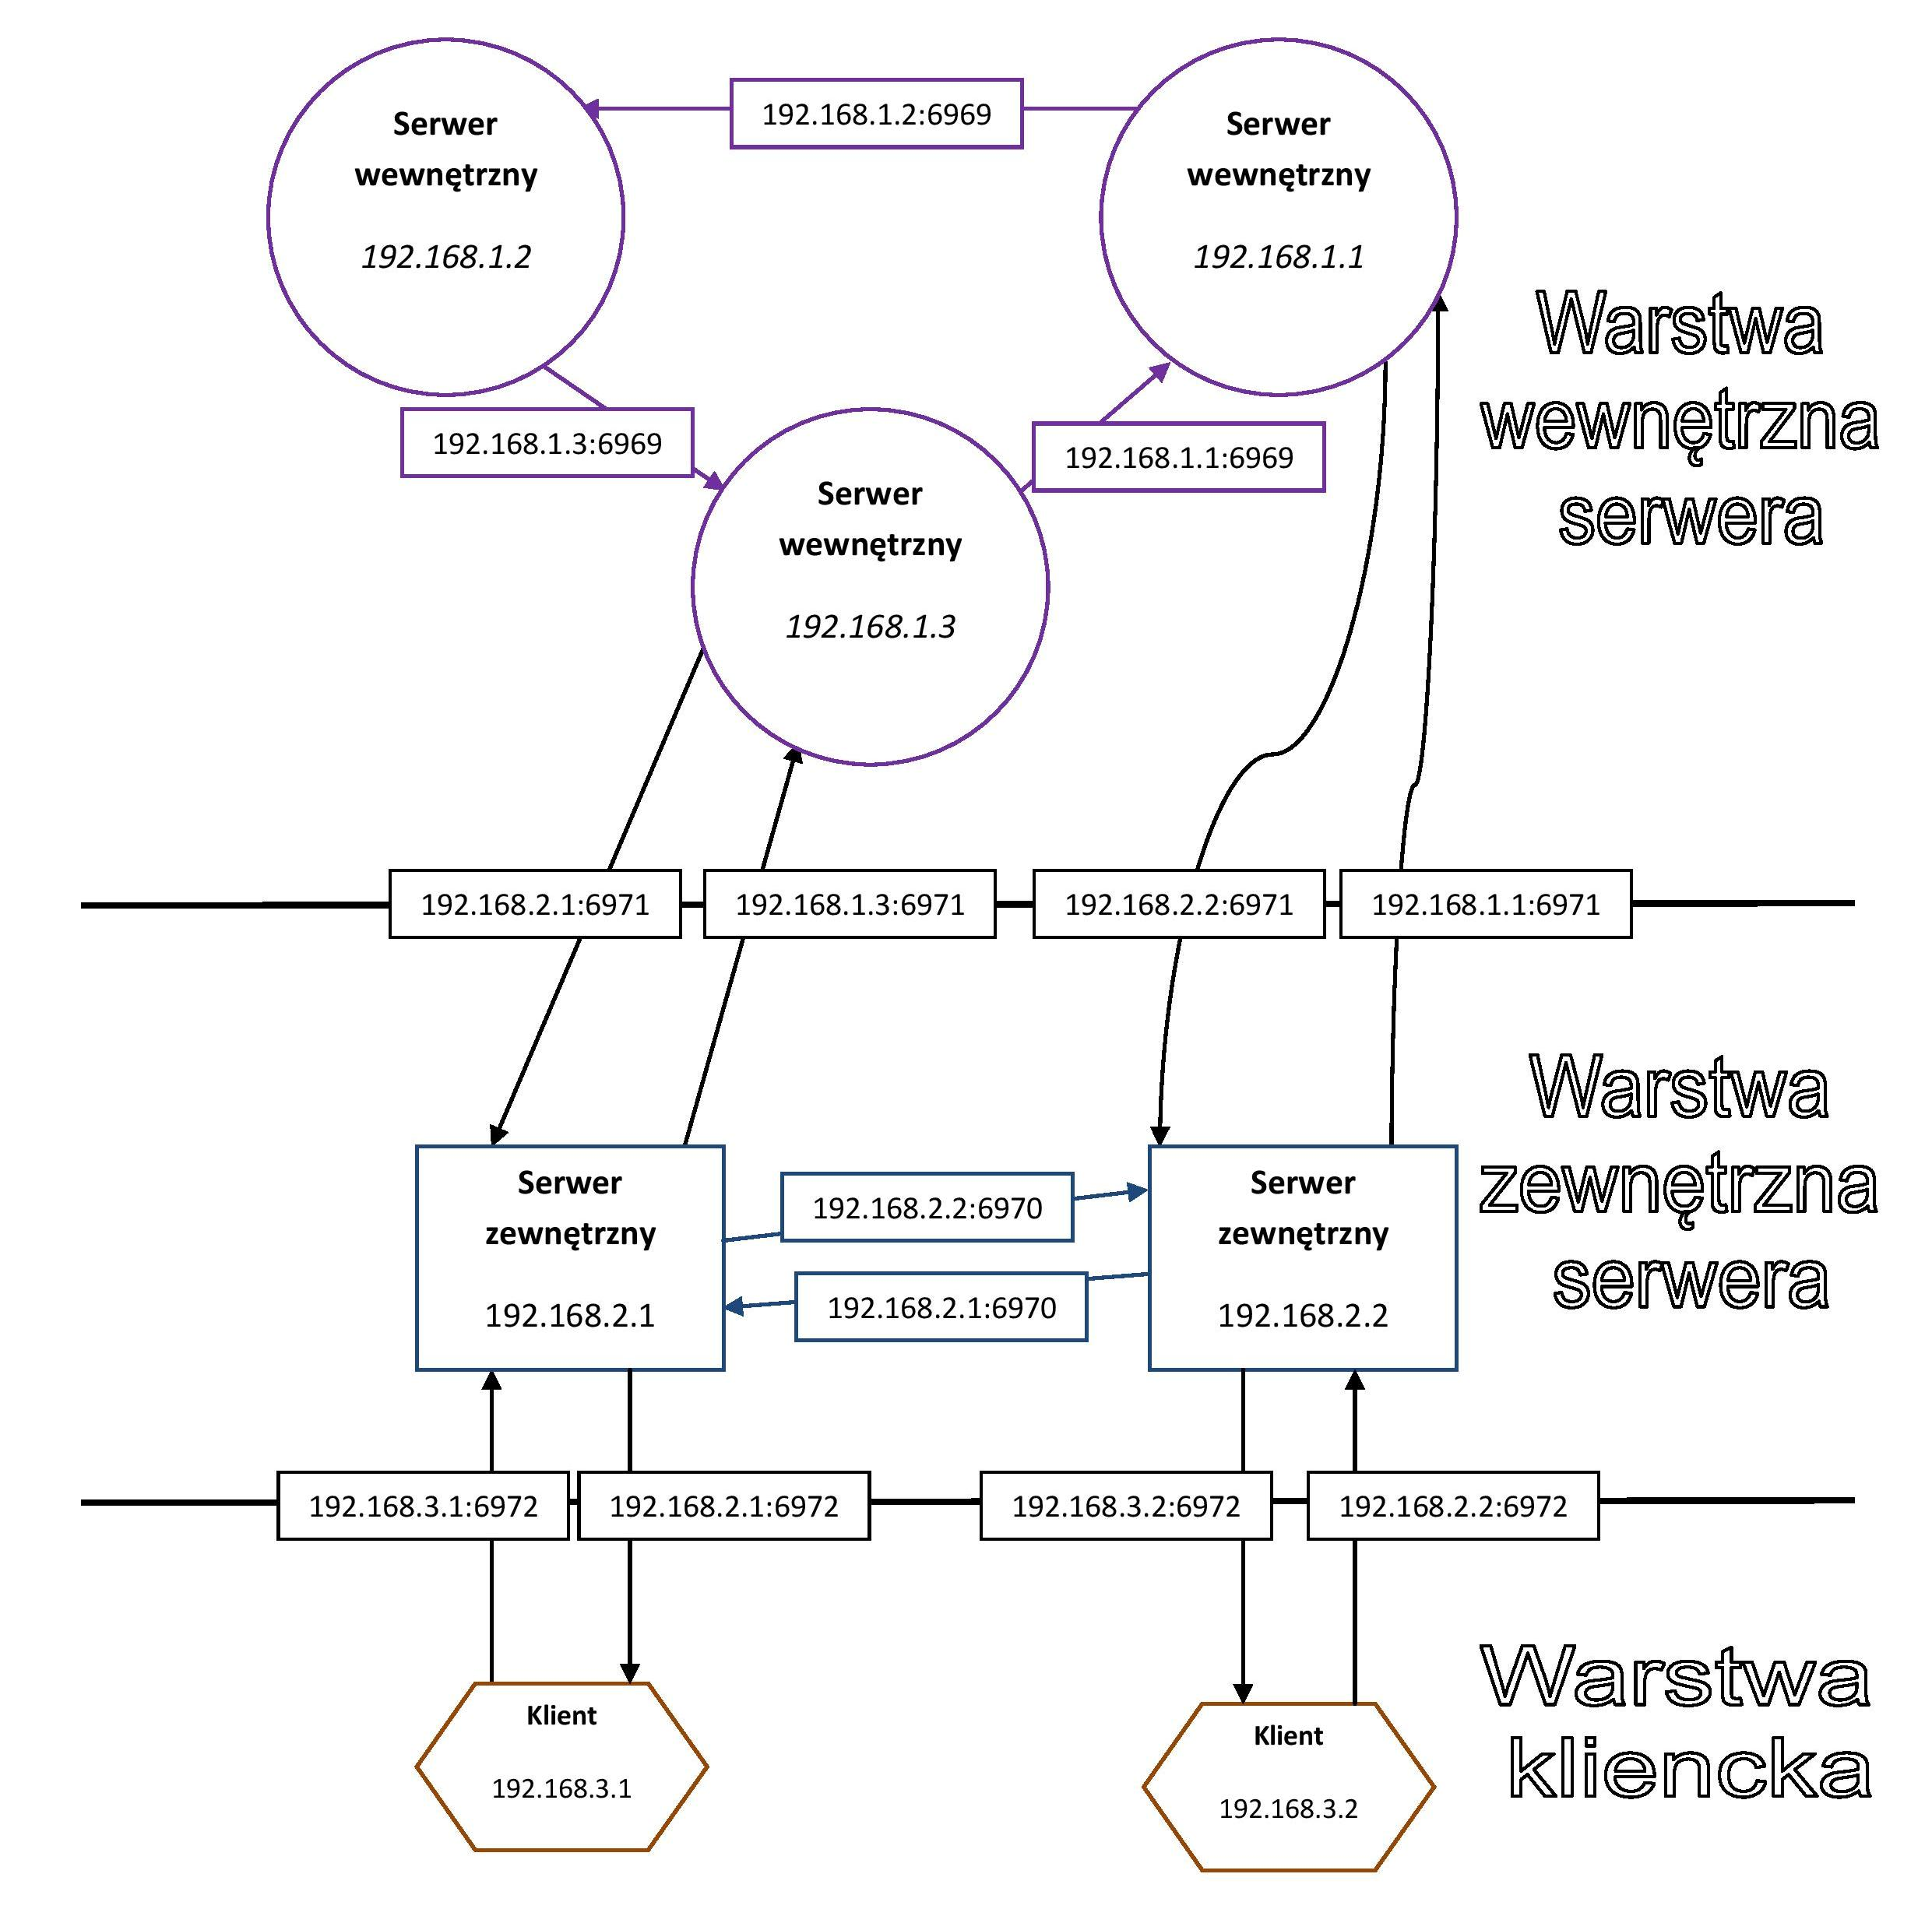
\includegraphics[width=0.9\linewidth]{img/komunikacja_schemat.jpg} 
\caption{Schemat komunikacji systemu}
\label{img:schem_kom}
\end{center}
\end{figure}

\textbf{Warstwa węwnętrzna (w obrębie warstwy)} \\
\textit{Wysyłanie i odbieranie danych} - na porcie 6969 \\

\textbf{Warstwa zewnętrzna (w obrębie warstwy)} \\
\textit{Wysyłanie i odbieranie danych} - na porcie 6970 \\


\textbf{Komunikacja między warstwą zewnętrzną a wewnętrzną} \\
\textit{Wysyłanie i odbieranie danych} - na porcie 6971 \\


\textbf{Komunikacja między warstwą zewnętrzną a klientem} \\
\textit{Wysyłanie i odbieranie danych} - na porcie 6972 \\




\subsection[Struktura pliku konfiguracyjnego]{Struktura pliku konfiguracyjnego}
\begin{lstlisting}
# RSO - konfiguracja

# Typ wezla.
# Mozliwe wartosci: server, middleware, client

rso.type = middleware

# Lista adresow IP wezlow
# Wartosci oddzielone przecinkami

rso.addresses = 127.0.0.1, 8.8.8.8, 192.168.1.1

# Port na ktorym dziala serwer wewnetrzny/zewnetrzny
# Wewnetrzny: 6969; Zewnetrzny :6970

rso.port.external = 6969

# Port na ktorym dziala serwer wewnetrzny/zewnetrzny: 6971;

rso.port.internal = 6969

# Port na ktorym laczy sie klient: 6972

rso.port.client = 6972

# Baza (nie dotyczy klienta)

jdbc.driverClassName=com.mysql.jdbc.Driver
jdbc.url=jdbc:mysql://localhost:3306/baza
jdbc.username=user
jdbc.password=haslo
init-db=false

# Czas timeoutu (w sekundach)
# Wewntrzny - oczekiwanie na token; Zewntrzny - oczekiwanie na Heartbeat
timeout = 30
\end{lstlisting}


\section[Potencjalne problematyczne scenariusze]{Potencjalne problematyczne scenariusze}

\begin{itemize}
\item \textbf{Podłączenie nowego serwera warstwy wewnętrznej}
\begin{itemize}
\item Brak innych aktywnych serwerów wewnętrznych
\item Jest aktywny przynajmniej jeden serwer wewnętrzny
\end{itemize}
\item \textbf{Podłączenie nowego serwera warstwy zewnętrznej i sprawdzanie aktywności pozostałych węzłów}
\begin{enumerate}
\item Próba połączenia z pozostałymi serwerami zewnętrznymi.
\item W razie udanego połączenia - serwer uznany za aktywny.
\item Od tej pory do każdego aktywnego serwera co określony interwał czasu wysyłany jest Heartbeat (chyba, że została wysłana jakakolwiek inna wiadomość). 
\item Analogicznie co ten sam interwał serwer oczekuje jakiejkolwiek wiadomości od aktywnych węzłów. Jeśli ich nie otrzyma - wysyła wiadomość TestRequest, żeby wymusić wysłanie Heartbeata od danego serwera. Jeśli serwer odpowie - nadal uznawany jest za aktywny - jeśli nie, uznawany jest od tego momentu za nieaktywny.
\end{enumerate}

\item \textbf{Awaria węzłów warstwy wewnętrznej serwera}
\begin{itemize}
\item Nie posiada tokena, brak zadań w toku, brak oczekujących zadań
\item Nie posiada tokena, brak zadań w toku, oczekujące zadanie od klienta
\item Nie posiada tokena, zadanie w toku
\item Posiada token, brak zadań w toku, brak oczekujących zadań
\item Posiada token, zadanie w toku, brak zadań w toku, oczekujące zadanie od klienta
\item Posiada token, zadanie w toku
\end{itemize}


\item \textbf{Awaria węzłów warstwy zewnętrznej serwera}
\par {Węzeł serwera może ulec awarii w sytuacji:}
\begin{enumerate}
\item Braku wykonywania konkretnych zadań
\par{W takim wypadku po rozłączeniu na dłużej niż określony interwał uznany jest przez pozostałe węzły za nieaktywny. Jeśli po krótkiej chwili połączy się ponownie - zostanie uznany za aktywny i cała warstwa będzie działała poprawnie. To samo tyczy się komunikacji serwera z klientami.}
\par {W przypadku awarii więcej niż jednego węzła na raz - algorytm nadal działa poprawnie (aż do awarii wszystkich serwerów).}

\item W trakcie wykonywania zapytania klienta
\par{Jeśli węzeł ulegnie awarii w trakcie wykonywania zapytania po określonym interwale klient próbuje się połączyć z innym serwerem (ponawiając proces logowania), jeśli to się powiedzie - ponawia zapytanie. Algorytm ten może mieć dość długi czas realizacji w porównaniu do wykonania samego zapytania (np. jeśli kolejny serwer, zgodnie z algorytmem wyrównującym obciążenie klientami serwerów zewnętrznych, zaproponuje serwer nieaktywny przez klienta) ale zapewnia odpowiednią synchronizację i stan całego systemu.}

\par{Jeśli serwer połączy się ponownie i wyśle odpowiedź do klienta - ten uzna ją za błąd i zgłosi to serwerowi. W tym momencie serwer ten wykreśla ze swojej listy danego klienta i dopisze do listy danego serwera (podanego w wiadomości). Następnie informacja ta zostanie spropagowana do innych serwerów (w Heartbeatach). Dzięki temu informacje lokalne na temat serwerów w warstwie będą poprawne.}

\par{Algorytm ten działa także w przypadku awarii większej liczby serwerów, lecz ma też w związku z tym dłuższy czas realizacji.}

\item W trakcie integracji z serwerem wewnętrznym

\end{enumerate}

\item \textbf{Kwestia równomiernego podziału klientów między serwery oraz serwerów zewnętrznych między wewnętrzne}
\begin{enumerate}
\item Wysłanie przez klienta wiadomości logowania do serwera
\item Serwer porównuje swoją ilość klientów do ilości klientów innych węzłów.
\item Jeśli serwer otrzymujący wiadomość po dodaniu kolejnego klienta NIE będzie miał przynajmniej o 2 więcej klientów od któregokolwiek innego serwera - loguje klienta, a algorytm zostaje zakończony.
\item Jeśli serwer otrzymujący wiadomość po dodaniu kolejnego klienta miałby przynajmniej o 2 więcej klientów od któregokolwiek innego serwera - wysyła klientowi informację z adresem serwera aktywnego o najmniejszej ilości podłączonych klientów. Klient ponawia logowanie do podanego serwera.
\end{enumerate}
\par{Algorytm zapewnia równomierne rozłożenie klientów pomiędzy aktywne serwery co wpływa pozytywnie na działanie i czas obsługi żądań przez system.}

\item \textbf{Kwestia rozmieszczenia warstw serwera w obrębie jednego komputera bądź wielu odrębnych}
\end{itemize}

\section[Ograniczenia i możliwe problemy]{Ograniczenia i możliwe problemy}
\textit{\textbf{TODO}}

\section[Organizacja środowiska programistycznego]{Organizacja środowiska programistycznego}

\subsection[Język programowania Java]{Język programowania Java}

\par{Zdecydowaliśmy się napisać kod źródłowy systemu w Javie. Wybór ten wynika z wielu zalet tego języka programowania. Funkcje sieciowe są dostępne w podstawowych bibliotekach. Wliczone w to są TCP/IP, UDP/IP, wydajne nieblokujące I/O, HTTP, wsparcie REST, XML, JSON oraz SSL.}

\par{Kolejną zaletą jest duży zbiór struktur danych (również w podstawowych bibliotekach). Budowa rozproszonego systemu wymaga wielu, często skomplikowanych i różnorodnych, struktur, które Java posiada. Ważna jest tu także kwestia wątków i synchronizacji między nimi. Na tym polu Java również dostarcza odpowiednie funkcje, struktury danych oraz narzędzie realizujące współdzielony dostęp. Ponadto bez problemu współpracuje z Google Protocol Buffers i jest multiplatformowa.}

\subsection[IntelliJ IDE]{IntelliJ IDE}

\par{Jest to środowisko programistyczne dla Javy. Owe środowisko wyposażono w bardzo bogatą paletę narzędzi pozwalających na komfortowe tworzenie oraz edycję kodu. Mnogość narzędzi oraz znajomość środowiska przez zespół ostatecznie zaważyła na decyzji o wykorzystaniu IntelliJ.}

